\documentclass[a4paper,12pt]{scrreprt}
\usepackage[code]{basis/optionen}

\addbibresource{literatur.bib}

\title{Mein Thema}
\author{Mein Name}
\date{01. Januar 1970}
\matrikelnr{111111}
\fach{Das Fach}
\professor{Der Professor}

\begin{document}

\pagenumbering{Roman}
\begin{titlepage}
\makeatletter
\begin{center}
    
\includegraphics[width=7cm]{basis/logo_hsan}
    
    \vspace{1em}
    
    \large{Fakultät Wirtschaft}
    
    \Large{Studiengang Wirtschaftsinformatik}
    
    \vspace{\stretch{1}}
    
    \huge{Studienarbeit}
    
    \vspace{\stretch{1}}
    
    \setlength{\fboxsep}{1em}
    \framebox[\textwidth]{
        \Huge{\textbf{\@title}}
    }
\end{center}

\vspace{\stretch{2}}

\begin{tabular}{@{} l l @{}}
Autor:             & \@author        \\
Matrikel-Nr.:      & \@matrikelnr    \\
                   &                 \\
Fach:              & \@fach          \\
Betreuung:         & \@professor     \\
                   &                 \\
Ort, Abgabetermin: & Ansbach, \@date
\end{tabular}

\vspace{\stretch{1}}

\makeatother
\end{titlepage}

\pdfbookmark[0]{\contentsname}{toc}
\tableofcontents
\listoffigures
\listoftables
\listoflistings
\addchap{Abkürzungsverzeichnis}
\begin{acronym}[IoT] %längste Abkürzung hier, damit Tabelle einheitlich formatiert wird
    %Hier Abkürzungen eintragen
    \acro{IoT}{Internet of Things}
\end{acronym}

\clearpage

\pagenumbering{arabic}
\onehalfspacing
%Hier eigenen Text schreiben 
\chapter{Einleitung}
Mein einführender Text

\chapter{Beispiele}
Hier stehen einige Beispiele zur Verwendung der Vorlage.

\section{Formatierung}
Text kann \textbf{fett}, \textit{kursiv} oder \texttt{monospaced} geschrieben werden.

\section{Zitieren}
JavaScript ist momentan die am weitesten verbreitete Programmiersprache \parencite{stackOverflowSurvey}.
Quellen werden in der Datei literatur.bib angegeben.

\section{Abkürzungen}
Um Abkürzungen wie \ac{IoT} zu verwenden, können diese in der Datei abkuerzungen.tex eingetragen werden.
So wird die Abkürzung bei der ersten Verwendung ausgeschrieben und automatisch ein Abkürzungsverzeichnis generiert.

\section{Abbildungen}
\begin{figure}[h]
    \centering
    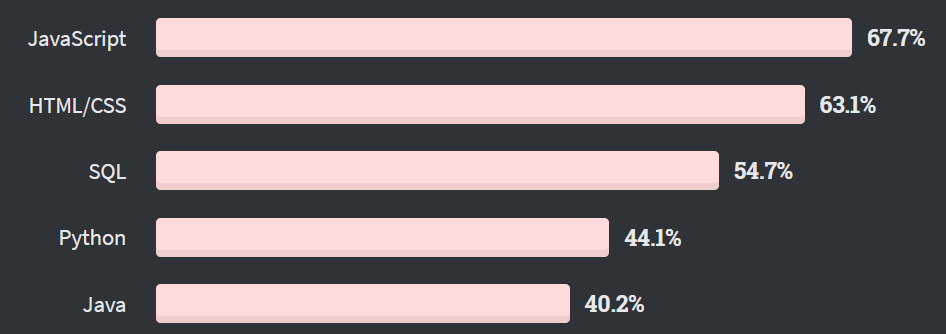
\includegraphics[width=\textwidth]{abbildungen/top5_languages.png}
    \caption{Die fünf beliebtesten Programmiersprachen \parencite{stackOverflowSurvey}}
    \label{fig:top5languages}
\end{figure}

Die Breite sollte entweder auf textwidth gesetzt werden, oder prozentual dazu z. B. mit 0.8textwidth verkleinert werden.
Die Caption sollte immer auch eine Quellenangabe mit parencite (eventuell mit dem Zusatz vgl.) erhalten.
Diese wird im Verzeichnis ausgeblendet.
Es kann auch im Text auf \autoref{fig:top5languages} verwiesen werden.

Um Quellcode einzubinden, sieht das Vorgehen ähnlich aus.

\begin{listing}[h]
    \inputminted{Java}{code/HelloWorld.java}
    \unskip
    \caption{Ein Hello World Programm in Java}
    \label{lst:helloworld}
\end{listing}


\chapter{Fazit}
Abschließende Worte

%Ende des eigenen Texts
\printbibliography
\chapter*{Eidesstattliche Erklärung}
\thispagestyle{empty}

Ich versichere, dass ich die Arbeit selbständig angefertigt, nicht anderweitig für Prüfungszwecke vorgelegt, alle benutzten Quellen und Hilfsmittel angegeben sowie wörtliche und sinngemäße Zitate gekennzeichnet habe.

\vspace{4em}

\begin{tabular}{@{} p{0.5\textwidth} l @{}}
..................................... & ..................................... \\
Ort, Datum                            & Unterschrift
\end{tabular}

\end{document}
